\subsection{The raster data model}

A raster is a data model constructed by a concise network of cells or pixels organised in a grid like structure \citep{bolstad_gis_2022,esri_raster}. Each cell in the raster is characterised by a cell-dimension, which defines the cell size by the cell length in X- and Y directions \citep{bolstad_gis_2022}. The cell size is therefore a representation of the rasters spatial resolution and serves as an indicator for the dataset's spatial precision. A larger cell size will return a higher spatial uncertainty, while smaller cell sizes do the opposite. However a smaller cell size entails a larger dataset. Using the raster-model is therefore a balancing act between good resolution and minimizing the size of the dataset.\\

Every cell has a value that represents information about the geographic location of the cell. This value can either be numerical or categorical, depending on the data represented. Numerical values are often used to describe continuous data such as elevation models, precipitation, and temperature.\\
Categorical values are used to represent discrete or thematic values where cells are classified into different categories. This is often done in LandUse/LandCover (LULC) datasets to represent forests or built up areas.\\

Important to note is that a cell also can have a unique value that represents "NoData". NoData is used when there is no information available and is useful when analysing specific cells. An advantage of NoData cells are that they are able to be used in logical expression to identify areas of NoData. However it is not possible to perform mathematical expressions on NoData values. All numerical calculations performed on a NoData cell will always return NoData. This issue can be mitigated by setting NoData values to a set value such as 0 or -9999 \citep{bolstad_gis_2022}.\\

\subsection{The Inundation Model}
To examine how a storm surge would impact a given area, a GIS-based storm surge screening-model, \textit{Inundation Model}, created by \cite{balstrom_kirby_inundation}. The model was developed to operate exclusively in ArcGIS Pro, the GIS software developed by American company ESRI.\\

The model and its framework consists of a multitude of tools to analyse a storms impact on an area. At the heart of the model is the tool \textit{"Create Inundation"}, which is static numerical raster model.\\
The model accepts three user defined numerical parameters as input. These three are: InitialSeaLevel, SeaLevelIncrement and Number of Iterations. InitialSeaLevel is the start value for initialisation, SeaLevelIncrement is the value the model increases by each iteration, and Number of Iterations is the amount of repetitions the model executes.\\
The calculation occurs over a hydrological corrected digital terrain model (DHyM) and a line geometry as source, called "LineAtSea" \citep{balstrom_kirby_inundation}. In figure \ref{Figur: Create Inundation} is the model's overall structure presented separated into two sections.
\begin{figure}[H]
	\centering
	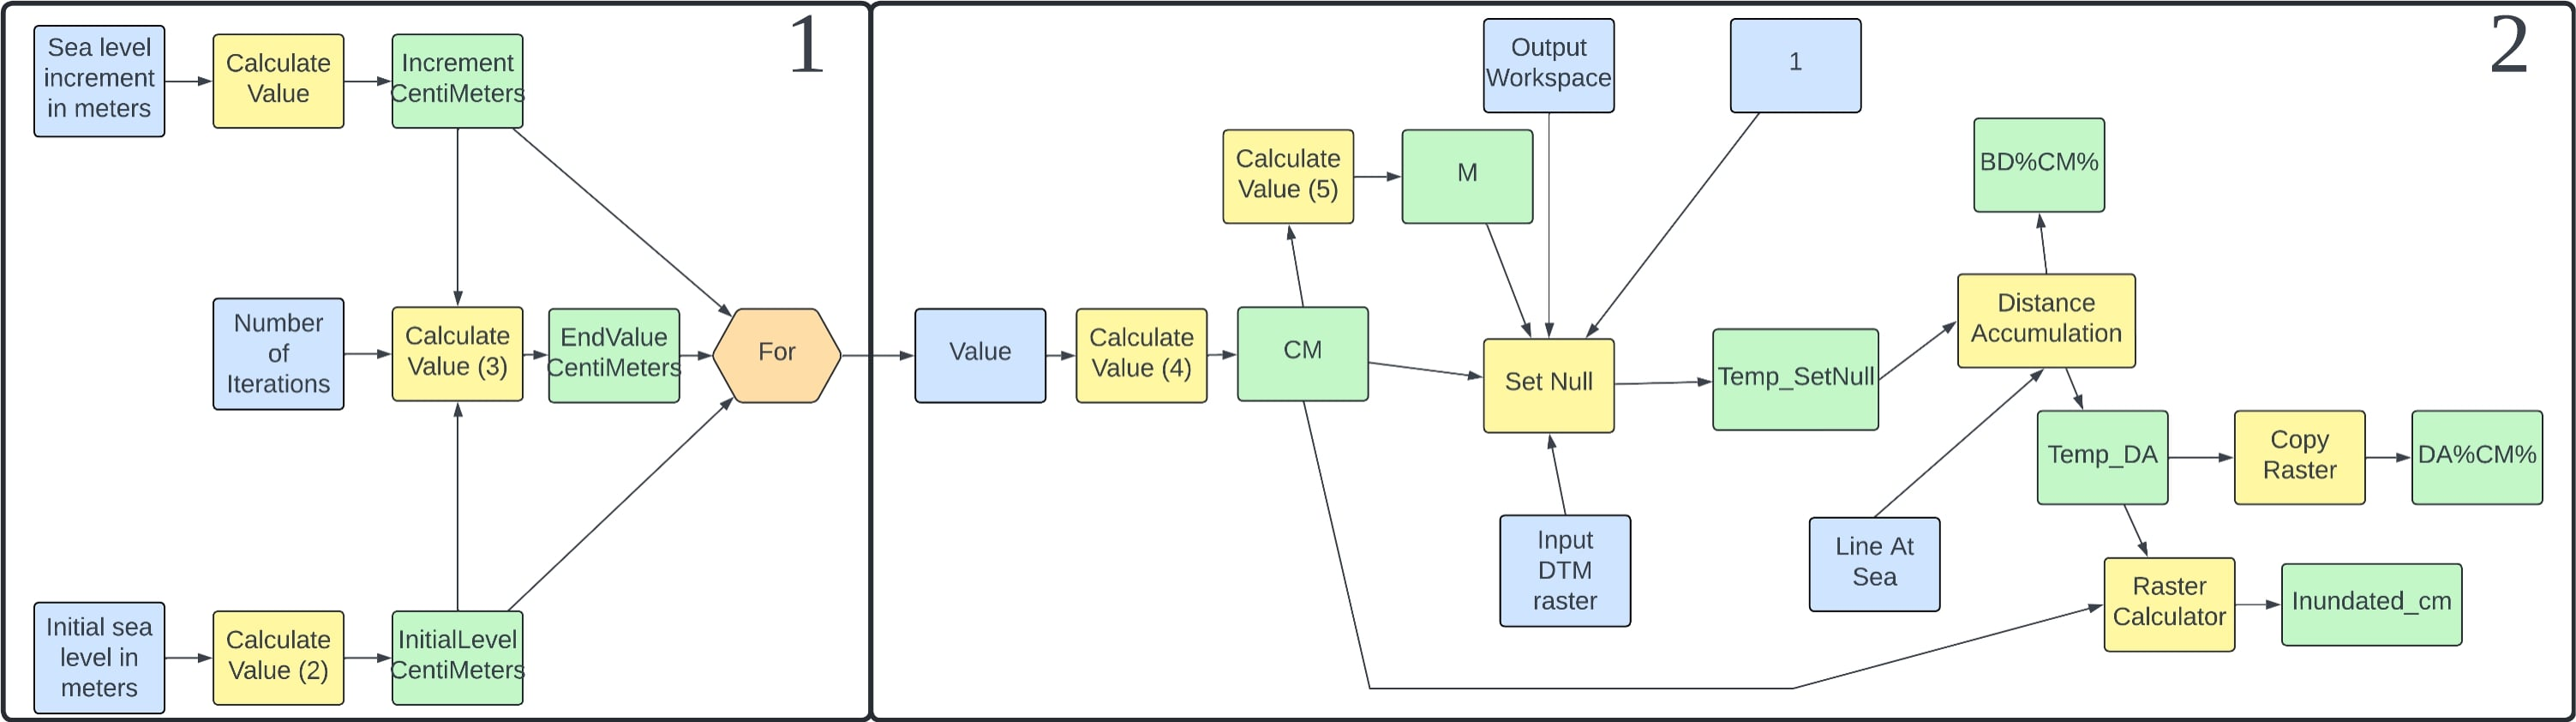
\includegraphics[width=1\linewidth]{images/teori/inundation_model_separated.jpg}
	\caption{Flowchart of the \textit{"Create Inundation"} tool in the Inundation Model}
	\label{Figur: Create Inundation}
\end{figure}
The first step is a recalculation of the input values from metres into centimetres. As well as a calculation for the end value of the model. This value is the stopping point for the models execution and is calculated as:\\ $InitialSeaLevel + ((Number of Iterations -1)\times Increment)$. Likewise it is possible to calculate the number of iterations based upon the desired end value: $(EndValue - InitialSeaLevel) / Increment - 1$.\\

The second part is a calculation through the terrain model (DTM). It is initialised by a for-loop that recalculates the centimetre value back to metres before executing a if-else statement on all the elevation values in the DTM. If the statement is true, then all values above current sea level iterated over will be assigned a NoData value, to indicate that the elevation cannot be flooded at that level. All other cells are assigned a 1. Figure \ref{Subfig: Celler Inundated} is a visual representation of this process. The cells in the DTM are not mutually exclusive in this process, so they will be assigned a 1 again in the next iteration.
\begin{figure}[H]
	\begin{subfigure}[t]{0.5\textwidth}
		\centering
		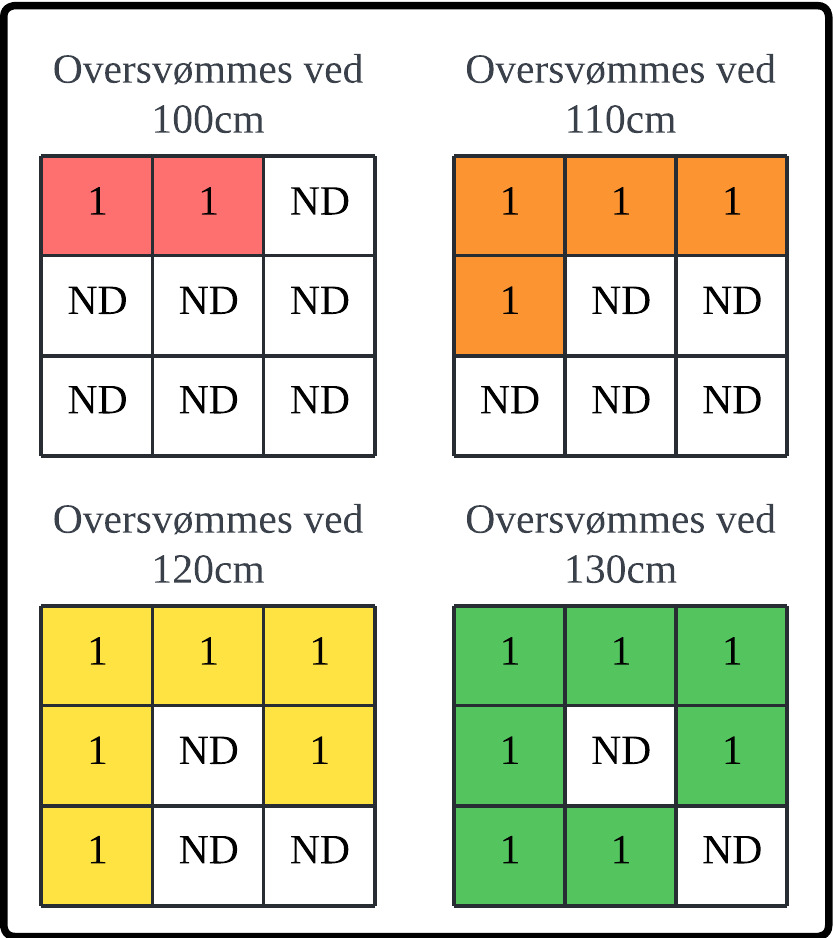
\includegraphics[width=0.7\linewidth]{images/teori/inundated_cells.jpeg}
		\caption{}
		\label{Subfig: Celler Inundated}
	\end{subfigure}
	\begin{subfigure}[t]{0.5\textwidth}
		\centering
		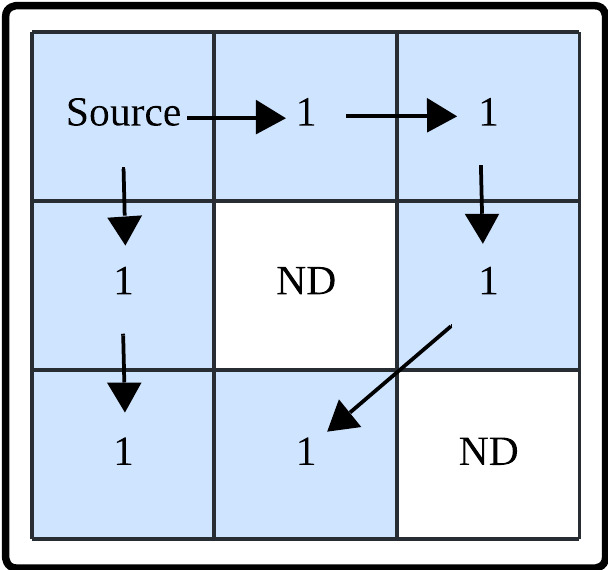
\includegraphics[width=0.85\linewidth]{images/teori/distance_accumulation.jpeg}
		\caption{}
		\label{Subfig: DA}
	\end{subfigure}
	\caption{The concept behind the Inundation Model. 1 = cells that can be flooded, ND = NoData (cells that cannot be flooded). \textbf{(a)} SetNull function determines which cells that can potentially be flooded at given water level. \textbf{(b)} Distance-Accumulation calculation from a point source through passable cells for a given water level. Source: Own illustration with inspiration from \cite{balstrom_kirby_inundation}.}
	\label{Figur: }
\end{figure}
A Distance Accumulation analysis is the performed through the cells that can be flooded, at the specified level, from the Line At Sea source. A Distance Accumulation (DA) is an analysis method that calculates the total accumulated distance of travel from a defined source through the cells of a raster \citep{esri_how_nodate}. In the Inundation Model, the DA is used to simulate the propagation of water through the terrain during a storm surge. DA continues through the passable cells until an impermeable barrier is encountered (figure \ref{Subfig: DA}). To spread through the cells in the DTM, an "eight-side" (D8) rule is used, which helps the algorithm determine which cells can be connected. The D8 rule tells the DA function to check for a passable cell in eight directions using bitwise encoded directions.\\

In the models workflow the DA analysis begins on a point on the \textit{"Line at Sea"} line marked as \textit{"Source"} in figure \ref{Subfig: DA} and travels through all cells equal to 1. If a cell is NoData, the analysis stops \citep{balstrom_kirby_inundation}. The result from the DA-analysis is the combined with the iterable sea level value to give the result of that iteration. The process then repeats until the end value is reached.